\documentclass{article}

\usepackage{times}
\usepackage{geometry}
\geometry{a4paper,left=0.6cm,right=0.7cm,top=1cm,bottom=1cm,columnsep=0.8cm}

\usepackage{fontawesome}
\usepackage[hidelinks]{hyperref}
\usepackage{multicol,paracol,tikz,hyphsubst,moresize,hyphenat,adjustbox,tabularx,xcolor,enumitem}
\newcolumntype{Y}{>{\RaggedRight\arraybackslash}X}
\setlist[itemize]{itemsep=1pt,leftmargin=*,topsep=-10pt}

\definecolor{maincolor}{HTML}{ffffff}
\definecolor{seccolor}{HTML}{0b1f3b}
\definecolor{gray}{HTML}{8c94a9}
\definecolor{sidetext}{HTML}{59cee5}
\definecolor{Green}{HTML}{2caf00}
\definecolor{lightgray}{HTML}{D3D3D3}

% --- bande latérale bleue
\usepackage{eso-pic}
\AddToShipoutPictureBG{%
  \begin{tikzpicture}[remember picture,overlay]
    \fill[seccolor] (0.7\paperwidth,0) rectangle (\paperwidth,\paperheight);
    \fill[maincolor] (0,0) rectangle (0.7\paperwidth,\paperheight);
  \end{tikzpicture}%
}

\setlength{\parindent}{0pt}
\newcommand{\cvsection}[1]{%
  \par\bigskip                % espace avant le titre
  {\bfseries\Large #1}\par
  \noindent\rule{\linewidth}{0.8pt}\par
  \medskip                    % espace après la ligne
}

\newcommand*{\ClipSep}{0.4cm}

% ------------------------------------------------------------------
\begin{document}\pagestyle{empty}
\columnratio{0.7}\begin{paracol}{2}

% --------- colonne gauche -----------------------------------------
\begin{minipage}{0.7\linewidth}
{\LARGE\textbf{Judikael Mourouvin}}

\bigskip
{\large\textbf{Technicien informatique \& marketing digital}}
\end{minipage}\hfill
\begin{minipage}{0.18\linewidth}
\begin{tikzpicture}
\node[inner sep=0pt]{ 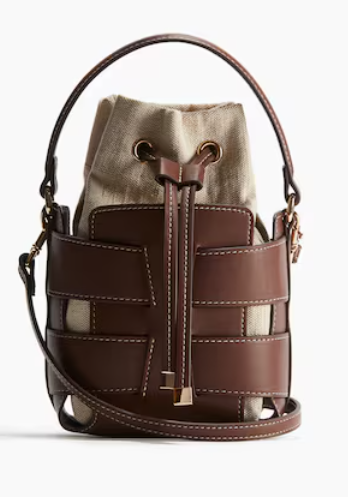
\includegraphics[width=\linewidth]{a52e10e7b6274df890fe899c2c0c3cbb.png} };
\draw[white,rounded corners=\ClipSep,line width=\ClipSep]
      (current bounding box.north west) --
      (current bounding box.north east) --
      (current bounding box.south east) --
      (current bounding box.south west) -- cycle;
\end{tikzpicture}
\end{minipage}

\cvsection{Profil}
Passionné par l’informatique et le marketing digital, je maîtrise la configuration de postes, la maintenance et le support utilisateurs. Mon année d’alternance à la DSI de la Mairie du Gosier m’a permis de gérer des projets numériques et de contribuer à la stratégie digitale. Rigoureux et orienté résultat, j’aspire désormais à rejoindre votre équipe à temps plein pour mettre mes compétences techniques et mon sens du service au profit de vos projets.

\cvsection{EXPÉRIENCE}

\colorbox{maincolor}{%
  \begin{minipage}{\linewidth}
    \textbf{Alternant en marketing digital} \\ Mairie du Gosier – DSI \\ 2023-2024
    \begin{itemize}
      \item Piloté des projets numériques en phase avec les objectifs de la collectivité. \item Analysé les besoins des usagers et déployé des solutions adaptées, améliorant l’expérience utilisateur. \item Assuré support et formations, renforçant la maîtrise des outils digitaux par les équipes.
    \end{itemize}
  \end{minipage}}

\vspace{3mm}


\colorbox{maincolor}{%
  \begin{minipage}{\linewidth}
    \textbf{Animateur de la zone informatique} \\ Pôle emploi, Gosier \\ 2022-2023
    \begin{itemize}
      \item Fournit un support quotidien aux collaborateurs, réduisant les interruptions de service. \item Configuré et entretenu le parc informatique, garantissant sa disponibilité optimale. \item Diagnostiqué puis résolu les incidents, maintenant un haut taux de disponibilité.
    \end{itemize}
  \end{minipage}}

\vspace{3mm}


\colorbox{maincolor}{%
  \begin{minipage}{\linewidth}
    \textbf{Stagiaire informaticien} \\ Numerika, Baie-Mahault \\ 2020-2021
    \begin{itemize}
      \item Installé et paramétré postes et périphériques, accélérant la mise en service. \item Apporté une assistance de proximité, résolvant rapidement les demandes utilisateurs.
    \end{itemize}
  \end{minipage}}

\cvsection{FORMATION}

    \begin{tabularx}{\linewidth}{@{}c >{\RaggedRight\arraybackslash}X@{}}
    \textcolor{sidetext}{\faGraduationCap} &
    \textbf{Bachelor Marketing Digital} \\
    & CFA IUTS \\
    & \textit{2023-2024} \\
    \end{tabularx}
    \begin{itemize}[leftmargin=*]
  \item Étude des stratégies de contenu, SEO/SEA et médias sociaux.
  \item Mise en place de campagnes digitales et analyse des performances.
  \item Gestion de projets marketing orientés acquisition et fidélisation.
\end{itemize}
\vspace{3mm}

    \begin{tabularx}{\linewidth}{@{}c >{\RaggedRight\arraybackslash}X@{}}
    \textcolor{sidetext}{\faGraduationCap} &
    \textbf{BTS Système Numérique option Informatique et Réseaux} \\
    & Lycée Chevalier Saint-Georges, Abymes \\
    & \textit{2019-2021} \\
    \end{tabularx}
    \begin{itemize}[leftmargin=*]
  \item Conception, installation et administration de réseaux locaux.
  \item Maintenance matérielle et logicielle de systèmes informatiques.
  \item Programmation et diagnostic d’incidents pour assurer la continuité de service.
\end{itemize}

% --------- colonne droite (bleue) ---------------------------------
\switchcolumn\color{white}\hspace*{0.4cm}\begin{minipage}{0.88\linewidth}

\cvsection{CONTACT}
\begin{tabular}{@{}c l}
  \faPhone & \href{tel:+590 0690 91 14 48}{+590 0690 91 14 48} \\[2pt]
  \faEnvelope & \href{mailto:jkmou971@gmail.com}{jkmou971@gmail.com} \\[2pt]
  \faMapMarker & Route de COCOYER\,97190 GOSIER \\[2pt]
  \faLinkedin & \href{}{}
\end{tabular}

\cvsection{COMPÉTENCES}

\begin{itemize}[leftmargin=*]
\item Administration
\item Réseaux
\item Support
\item Maintenance
\item Configuration
\item Diagnostic
\item Marketing\end{itemize}
\par\bigskip 

\cvsection{LANGUES}
\begin{itemize}[leftmargin=*]
\item English - \textcolor{gray}{}
\item Espagnol - \textcolor{gray}{}\end{itemize}
\par\bigskip 
\cvsection{INTÉRÊTS}
\begin{itemize}[leftmargin=*]
\item Lectur
\item Sports
\item Musique
\item Voyage
\end{itemize}

\end{minipage}
\end{paracol}
\end{document}
